\documentclass{article}
\usepackage[a4paper,left=2.5cm,right=2.5cm,top=2.5cm,bottom=2.5cm]{geometry}

\title{Session 3}
\author{Zohaad Fazal}
\date{February 2020}
\usepackage{amsmath}
\usepackage{amssymb}
\usepackage{bbm}
\usepackage{tikz}
\usepackage{tkz-euclide}
\usetkzobj{all}
\usepackage{cancel}
\usepackage{caption}
\usepackage{textcomp}
\usepackage{eurosym}


\usetikzlibrary{calc,intersections,through,backgrounds,matrix,patterns}
\usepackage{pgfplots}
\usepgfplotslibrary{fillbetween}
\pgfdeclarelayer{bg}
\pgfsetlayers{bg,main}

\tikzset{
    hatch distance/.store in=\hatchdistance,
    hatch distance=10pt,
    hatch thickness/.store in=\hatchthickness,
    hatch thickness=0.3pt
}

\makeatletter
\pgfdeclarepatternformonly[\hatchdistance,\hatchthickness]{northeast}
{\pgfqpoint{0pt}{0pt}}
{\pgfqpoint{\hatchdistance}{\hatchdistance}}
{\pgfpoint{\hatchdistance-1pt}{\hatchdistance-1pt}}%
{
    \pgfsetcolor{\tikz@pattern@color}
    \pgfsetlinewidth{\hatchthickness}
    \pgfpathmoveto{\pgfqpoint{0pt}{0pt}}
    \pgfpathlineto{\pgfqpoint{\hatchdistance}{\hatchdistance}}
    \pgfusepath{stroke}
}

\pgfdeclarepatternformonly[\hatchdistance,\hatchthickness]{northwest}
{\pgfqpoint{0pt}{0pt}}
{\pgfqpoint{\hatchdistance}{\hatchdistance}}
{\pgfpoint{\hatchdistance-1pt}{\hatchdistance-1pt}}%
{
    \pgfsetcolor{\tikz@pattern@color}
    \pgfsetlinewidth{\hatchthickness}
    \pgfpathmoveto{\pgfqpoint{\hatchdistance}{0pt}}
    \pgfpathlineto{\pgfqpoint{0pt}{\hatchdistance}}
    \pgfusepath{stroke}
}



% derivative symbol
\renewcommand{\d}[1]{\ensuremath{\operatorname{d}\!{#1}}}

\newcommand{\notimplies}{%
  \mathrel{{\ooalign{\hidewidth$\not\phantom{=}$\hidewidth\cr$\implies$}}}}

\begin{document}

\maketitle

\section*{0\quad Topics}
\begin{enumerate}
    \item Pareto Optimality \& VMP (vector maximum problem)
    \item Inefficiency of equilibrium
    \item Common value auctions
    \item Revenue maximization
\end{enumerate}

\section{Pareto Optimality \& VMP}
$N=\{1,\dots,n\}$ agents, $A$ set of allocations
\begin{equation*}
\begin{aligned}
    & v_i:A\to \mathbb{R}\quad & \text{valuation function of agent } i.\\
    & a\mapsto v_i(a)\quad & \text{valuation of agent $i$ for allocation $a$.}
\end{aligned}
\end{equation*}
\subsection*{Pareto Optimality}
$a,b\in A$\\

\noindent
$b$ Pareto dominates $a$ if $v_i(b)\geq v_i(a)$ for all $i\in N$ with strict
inequality for at least one $j\in N$.\\

\noindent
$a$ is Pareto undominated (also: Pareto optimal, efficient) if there is no allocation $b\in A$ that Pareto dominates $a$.

\subsection*{TU (Total Utility)}
For $a\in A$

\begin{equation*}
    TU(a)=\sum_{i\in N}v_i(a)
\end{equation*}
\noindent
$a$ is TU maximizer if
\begin{equation*}
    TU(a)\geq TU(b)\quad\text{for all }b\in A
\end{equation*}
\\
\noindent
\textbf{Fact:} If $a$ is a TU maximizer, then $a$ is efficient.\\

\noindent
\textit{Proof:} by contradiction, assume $a$ is not efficient. There exists a $b\in A$ such that $v_i(b)\geq v_i(a)$ for all $i\in N$ and $v_j(b)>v_j(a)$ for at least one $j\in N$. $\sum_{i\in N} v_i(b)>\sum_{i \in N} v_i(a)\implies TU(b)>TU(a)$, so $a$ is not a TU maximizer, this is a contradiction.\\

\noindent
Note: Pareto undominated $\notimplies$ TU maximizer, here's an example:


\begin{table}
    \centering
    \begin{tabular}{c|c|c|c|c|c|c}
    allocation & 1 & 2 & 3 & 4 & 5 & TU \\ \hline
    $a_1$      & 3 & 2 & 0 & 4 & 2 & 11 \\
    $a_2$      & 2 & 1 & 4 & 3 & 1 & 11 \\
    $a_3$      & 4 & 2 & 1 & 4 & 3 & 14 \\
    $a_4$      & 3 & 2 & 1 & 4 & 2 & 12 \\
\end{tabular}
\caption*{$a_2$ and $a_3$ are Pareto undominated}
\end{table}
\newpage

\subsection*{Quasi-linear utility}
\begin{equation*}
    u_i(a,p)=v_i(a)-p
\end{equation*}
\noindent
Quasi-linear because it's only linear in $p$ and not in $a$.\\

\noindent
\textbf{Fact:} Under quasi-linear utility, Pareto optimality is equivalent to TU maximization.\\
\noindent
This is called the no wealth effect, in the real world there is a wealth effect: you're happier with \euro 100 if you were broke than if you were a millionaire.\\

\noindent
In the context of the example above, assume quasi-linear utility and money transfers. Then $a_3$ + money transfers Pareto dominates $a_2$. An example: P1 and P5 both pay \euro 1.50 to P3.\\

\begin{center}
\begin{tabular}{c|ccccc|c}
    player & 1 & 2 & 3 & 4 & 5 & TU\\ \hline
    $a_3$ & 4 & 2 & 1 & 4 & 3 & 14 \\
    new allocation & 2.5 & 2 & 4 & 4 & 1.5 & 14 \\
    calculations of payments & (4-1.5) & & (1+3) & & (3-1.5) & 
\end{tabular}
\end{center}

\noindent
If there is quasi-linear utility and enough money for money transfers, you can always take the TU maximizer and make it Pareto dominate any other allocation (not all other allocations simultaneously though). Here's an example with 2 agents and 6 allocations:

\begin{center}
\begin{tikzpicture}[scale=1.5]
\draw[thick,->] (0,0) -- (3,0) node[anchor=north west] {$u_1$} node[anchor=north east] {};
\draw[thick,->] (0,0) -- (0,3) node[anchor=south east] {$u_2$} node[anchor=north east] {};
\tkzDefPoint(0.5, 1){A};
\tkzDefPoint(1, 0.5){B};
\tkzDefPoint(1.75,0.7){C};
\tkzDefPoint(0.75,2.7){D};
\tkzDefPoint(2.5,0.5){E};
\tkzDefPoint(2,3){F};

\node at (F)[anchor=south west] {\; TU maximizer}; 
\node at (E)[anchor=south west] {\; undominated area};

% 45 degree arrows
\draw[dashed, ->] (2,3) -- (3,2);
\draw[dashed, ->] (2,3) -- (1,4);

% undominated arrows
\draw[dashed, ->] (2.5,0.5) -- (2.5,2.8);
\draw[dashed, ->] (2.5,0.5) -- (5,0.5);

\foreach \n in {A,B,C,D,E,F}
  \node at (\n)[circle,fill,inner sep=1.5pt]{};


\end{tikzpicture}
\end{center}

When the TU maximizer with money transfers Pareto dominates the undominated allocation, another allocation, the one at the top left, becomes undominated.

\section{Inefficiency of equilibrium}
\subsection*{Bilateral trade}
2 agents: buyer and seller. 1 indivisible item currently owned by seller.
\begin{equation*}
\begin{aligned}
    &v_B\in[0,1]\\
    &v_S\in[0,1]
\end{aligned}
\end{equation*}
The valuations are assumed to be iid draws from $U[0,1]$.\\

\noindent
\textbf{Efficiency:} Trade $\iff v_B\geq v_S$.\\
\noindent
\textbf{Information asymmetry:} $v_B, v_S$ are private.\\

\noindent
\textbf{Theorem: Myerson}\\
There is no mechanism with an equilibrium in which allocation is efficient (Pareto optimal).\\
\textit{Proof:} not going to prove this.

\subsection*{Double auction}
Bid of buyer $p_B \in[0,1]$, bid of seller $p_S\in[0,1]$. Think of these as functions of the valuations; $p_B(v_B)$ and $p_S(v_S)$. Trade $\iff p_B\geq p_S$. The payment from buyer to seller is determined by

\begin{equation*}
    p=\frac{p_B+p_S}{2}
\end{equation*}
\textbf{Example:} ex post equilibrium\\
\noindent

Given some exogenous threshold, $x\in[0,1]$, the bid profiles are
\begin{equation*}
        p_B(v_B)=
        \begin{cases}
            x&\text{if }v_B\geq x\\
            0&\text{if }v_B<x
        \end{cases}
        ,\quad p_S(v_S)=
        \begin{cases}
            1&\text{if }v_S>x\\
            x&\text{if }v_S\leq x
        \end{cases}
\end{equation*}
\textbf{Claim:} This is an ex post equilibrium\\
\noindent
\textit{Proof:}\\
If $v_B\geq x$ and $v_S \leq x$, the buyer is facing $p_S=x$, the buyer faces the following scenario:
\begin{equation*}
\begin{aligned}
    &\text{if }p_B<x,\quad u_B=0\\
    &\text{if }p_B\geq x,\quad u_B=v_B-\frac{p_B+x}{2}
\end{aligned}
\end{equation*}

The buyer will bid $p_B=x$ to maximize $u_B$.\\
Etc. There are in total 8 cases, 4 for the buyer and 4 for the seller.\\

\noindent
\textbf{Efficiency}
\begin{center}
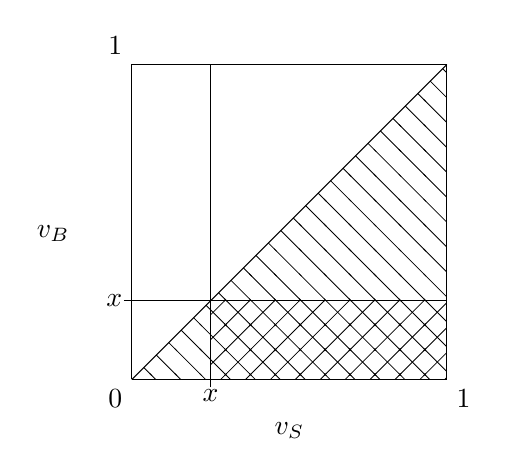
\begin{tikzpicture}
\draw (0,0) -- (4,0) node[anchor=north west]{1} node[label={[xshift=-2cm, yshift=-1cm]$v_S$}] {} -- (4,4) -- (0,4) node[anchor=south east]{1} -- (0,0) node[anchor=north east]{0} node[label={[xshift=-1cm, yshift=1.5cm]$v_B$}] {};

% diagonal
\draw (0,0) -- (4,4);

% x lines
\draw (0,1) -- (4,1);
\draw (1,0) -- (1,4);

% axis x labels
\draw (-0.1,1) -- (0,1) node[anchor=east] {$x$};
\draw (1, -0.1) -- (1,0) node[anchor=north] {$x$};

\begin{pgfonlayer}{bg}
% triangle pattern
\pattern[black, pattern=northwest, pattern color=black, hatch distance=10pt] (0,0)--(4,4)--(4,0);
% square pattern
\pattern[black, pattern=northeast, pattern color=black, hatch distance=10pt] (1,0)--(1,1)--(4,1)--(4,0);
\end{pgfonlayer}

\end{tikzpicture}
\end{center}
Efficiency dictates trade should happen in the dashed area, but it does not. Trades only happen where the cross pattern is.

\section{Common value auctions}
\subsection*{Economics}
$n=2$, 1 indivisible item, $v$ common value. Private signals, $s_1\in[0,1]$ and $s_2\in[0,1]$ iid draws from $U[0,1]$. There is a common valuation:
\begin{equation*}
    v=s_1+s_2
\end{equation*}
It's a 1\textsuperscript{st} price, sealed bid auction.\\

\noindent
\textbf{Bayesian Nash Equilibrium}\\
\begin{equation*}
\begin{aligned}
    b_1(s_1)=c\cdot s_1\\
    b_2(s_2)=c\cdot s_2
\end{aligned}
\end{equation*}
Bidder 1 has signal $s_1$ and knows bidder 2 bids according to $b_2(s_2)=c\cdot s_2$. Bidder 1 bids $b$, what should $c$ be? Maximize expected utility:
\begin{equation*}
    \begin{aligned}
        \mathbb{E}[\text{utility}]&=\mathbb{E}[v-b|\text{you win}]\cdot\mathbb{P}[\text{you win}]\\
        &= \mathbb{E}[s_1+s_2-b|b>c\cdot s_2]\cdot\mathbb{P}[b>c\cdot s_2]\\
        &=\left(s_1 + \mathbb{E}\left[s_2|s_2<\frac{b}{c}\right]-b\right)\cdot\mathbb{P}\left[s_2<\frac{b}{c}\right]\\
        &=\left(s_1+\frac{b}{2c}-b\right)\cdot\frac{b}{c}
    \end{aligned}
\end{equation*}
The first order condition is:
\begin{equation*}
    \begin{aligned}
        \frac{1}{c}\left(s_1+\frac{b}{2c}-b\right) + \left(\frac{1}{2c}-1\right)\cdot\frac{b}{c}&=0\\
        (2cs_1+b-2cb)+(1-2c)\cdot b&=0 \quad(\text{multiplied with }2c^2)\\
        2cs_1&=-b+2cb-b+2cb\\
        cs_1&=-b+2cb\\
        b&=\frac{c}{2c-1}\cdot s_1
    \end{aligned}
\end{equation*}
Because of symmetry:
\begin{equation*}
    \begin{aligned}
        \frac{c}{2c-1}&=c\\
        c=0\quad\text{or}&\quad c=1
    \end{aligned}
\end{equation*}

\section{Revenue maximization}
$n=2$, 1 indivisible item, $v_1\in[0,1]$ and $v_2\in[0,1]$ are iid draws from $U[0,1]$, $r$ reservation value. It is a 2\textsuperscript{nd} price, sealed bid plus reserve auction. If both bids are above $r$, it's a regular Vickrey auction. If one of the bids is lower, the winner pays $r$. If both are lower, the item doesn't get allocated. The idea is to sacrifice efficiency to increase expected revenue.\\

\noindent
In this auction, $b_1(v_1)=v_1$ and $b_2(v_2)=v_2$ is a DSE (dominant strategy equilibrium). The proof is easy, view the reserve price as the auctioneer playing as an extra bidder who always bids $r$. The DSE is still $b_i(v_i)=v_i$ for all $i\in N$. The payoff diagram for the auctioneer:

\begin{center}
\begin{tikzpicture}
\draw (0,0) -- (4,0) node[anchor=north west]{1} node[label={[xshift=-2cm, yshift=-1cm]$v_2$}] {} -- (4,4) -- (0,4) node[anchor=south east]{1} -- (0,0) node[anchor=north east]{0} node[label={[xshift=-1cm, yshift=1.5cm]$v_1$}] {};

% diagonal
\draw (1,1) node[label={[xshift=-0.5cm, yshift=-0.8cm]0}]{} -- (4,4) node[label={[xshift=-2cm, yshift=-1.5cm]$2,v_1$}]{} node[label={[xshift=-1cm, yshift=-2.5cm]$1,v_2$}]{};

% x lines
\draw (0,1) -- (4,1) node[label={[xshift=-1.6cm, yshift=-0.9cm]$1,r$}]{};
\draw (1,0) -- (1,4) node[label={[xshift=-0.5cm, yshift=-2cm]$2,r$}]{};

% axis x labels
\draw (-0.1,1) -- (0,1) node[anchor=east] {$x$};
\draw (1, -0.1) -- (1,0) node[anchor=north] {$x$};
\end{tikzpicture}
\end{center}

\begin{equation*}
    \begin{aligned}
        \mathbb{E}[\text{revenue}]&=2r(1-r)\cdot r+2\cdot\int_r^1\int_{v_1}^1v_1\d v_2 \d v_1\\
        &=2r^2(1-r)+2\cdot\int_r^1v_2(1-v_2)\d v_1\\
        &=2r^2(1-r)+\left[\frac{1}{2}v_1^2-\frac{1}{3}v_1^3\right]_r^1\\
        &=2r^2-2r^3+2\left(\frac{1}{6}-\frac{1}{2}r^2+\frac{1}{3}r^3\right)\\
        &=\frac{1}{3}+r^2-\frac{4}{3}r^3
    \end{aligned}
\end{equation*}
Sanity check: for $r=0$, $\mathbb{E}[\text{revenue}]=\frac{1}{3}$, which is the same as the expected revenue of the Vickrey auction (2\textsuperscript{nd} price, sealed bid auction). For $r=1$, $\mathbb{E}[\text{revenue}]=0$, which is logical, no one will win because the auctioneer bids the maximum bid.\\

\noindent
First order condition
\begin{equation*}
    \begin{aligned}
        2r-4r^2&=0\\
        2r(1-2r)&=0\\
        r=0\quad\text{or}\quad &r=\frac{1}{2}
    \end{aligned}
\end{equation*}

\noindent
For $r=0$, $\mathbb{E}[\text{revenue}]=\frac{1}{3}$, for $r=\frac{1}{2}$, $\mathbb{E}[\text{revenue}]=\frac{1}{3} + \left(\frac{1}{2}\right)^2-\frac{4}{3}\left(\frac{1}{2}\right)^3=\frac{5}{12}$. As $\frac{5}{12}>\frac{1}{3}$, the auctioneer can expect more revenue by setting $r=\frac{1}{2}$.

\begin{center}
\begin{tikzpicture}[scale=4]
      \draw[->] (-0.5,0) -- (1.5,0) node[right] {$r$};
      \draw[->] (0,-0.5) -- (0,1) node[above] {$\mathbb{E}[\text{revenue}]$};
      \draw[scale=1,domain=0:1,smooth,variable=\x] plot ({\x},{\x*\x - 4/3*\x*\x*\x + 1/3});
      \draw[scale=1,domain=-0.5:0,smooth,variable=\x,dashed] plot ({\x},{\x*\x - 4/3*\x*\x*\x + 1/3});
      \draw[scale=1,domain=0:1.2,smooth,variable=\x,dashed] plot ({\x},{\x*\x - 4/3*\x*\x*\x + 1/3});
      \draw (1/2-1/4,5/12) -- (1/2+1/4,5/12) node[right] {$\frac{5}{12}$};
      \draw (0+1/4,1/3) -- (0-1/4,1/3) node[left] {$\frac{1}{3}$};
      \node[below left] at (0,0) {0};
      \draw (1/2,0) -- (1/2,-0.05) node[below] {$\frac{1}{2}$};
      \node[below left] at (1,0) {1};
\end{tikzpicture}    
\end{center}


\end{document}
